\begin{frame}{データセットの下準備}{手法：時間の切り方}
  \lead{時間は「半月」で切る。データが支える最も細かい単位は 15 日}
  \begin{columns}[T]
    \begin{column}{0.40\textwidth}
      \begin{center}
      \begin{tikzpicture}[x=1mm,y=1mm]
        \fill[wcPale] (0,0) rectangle (25,6.5);
        \fill[wcBlue!25] (25,0) rectangle (50,6.5);
        \draw[wcMuted,line width=0.5pt] (0,0) rectangle (50,6.5);
        \draw[wcBlue,line width=0.9pt] (25,0) -- (25,6.5);
        \node[font=\mediumfont\fontsize{10}{12}\selectfont,text=wcText] at (12.5,3.25) {前半 1--15 日};
        \node[font=\mediumfont\fontsize{10}{12}\selectfont,text=wcText] at (37.5,3.25) {後半 16 日--月末};
      \end{tikzpicture}
      \end{center}
      \vskip 0.5mm
      \sub{1 年抜きの交差検証（10 通り）}
      \vskip -1.5mm
      \[
        \text{誤差の削減} = 1 - \frac{\mathrm{RMSE}}{\mathrm{RMSE}_{\text{季節なし}}}
      \]
      \vskip -3mm
      \sub{2 SE 以内は区別できない \src{Hastie+09}}
    \end{column}
    \begin{column}{0.58\textwidth}
      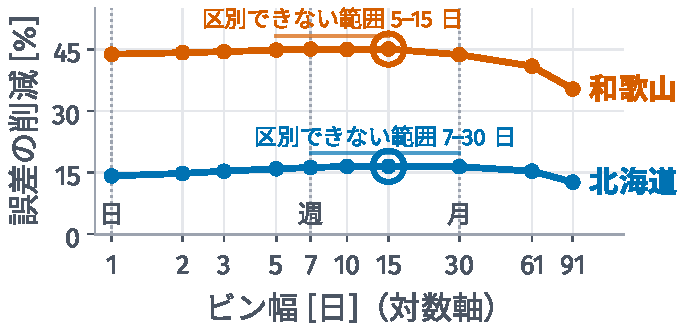
\includegraphics[width=\linewidth,height=136pt,keepaspectratio]{S_skill_overlay.pdf}
    \end{column}
  \end{columns}
  \srcline{年 24 ビン、各 520--640 解析値。落下位置のベクトル RMSE、2016--2025}
\end{frame}
